\subsubsection{Expansion Parallel Port}

The {\it \systemNameFull} includes two bidirectional parallel ports that are connected to the
{\it \expansionPortA} and {\it \expansionPortB} 40-pin headers on the \DEBoard~board. These parallel ports
include the four 32-bit registers that were described previously for 
Figure~\ref{fig:parallel_port}. The base address of the port for \expansionPortA~is {\sf 0xFF200060},
and for \expansionPortB~is {\sf 0xFF200070}.  Figure~\ref{fig:expansion_port} gives a diagram of 
the 40-pin connectors on the \DEBoard~board, and shows how the respective parallel port {\it Data} register bits, 
$D_{31-0}$, are assigned to the pins on the connector. The figure shows that bit $D_0$ of
the parallel port is assigned to the pin at the top right corner of the
connector, bit $D_1$ is assigned below this, and so on. Note that some of the pins on
the 40-pin header are not usable as input/output connections, and are 
therefore not used by the parallel ports. Also, only 32 of the 36 data pins that appear on
each connector can be used.

\begin{figure}[h!]
   \begin{center}
       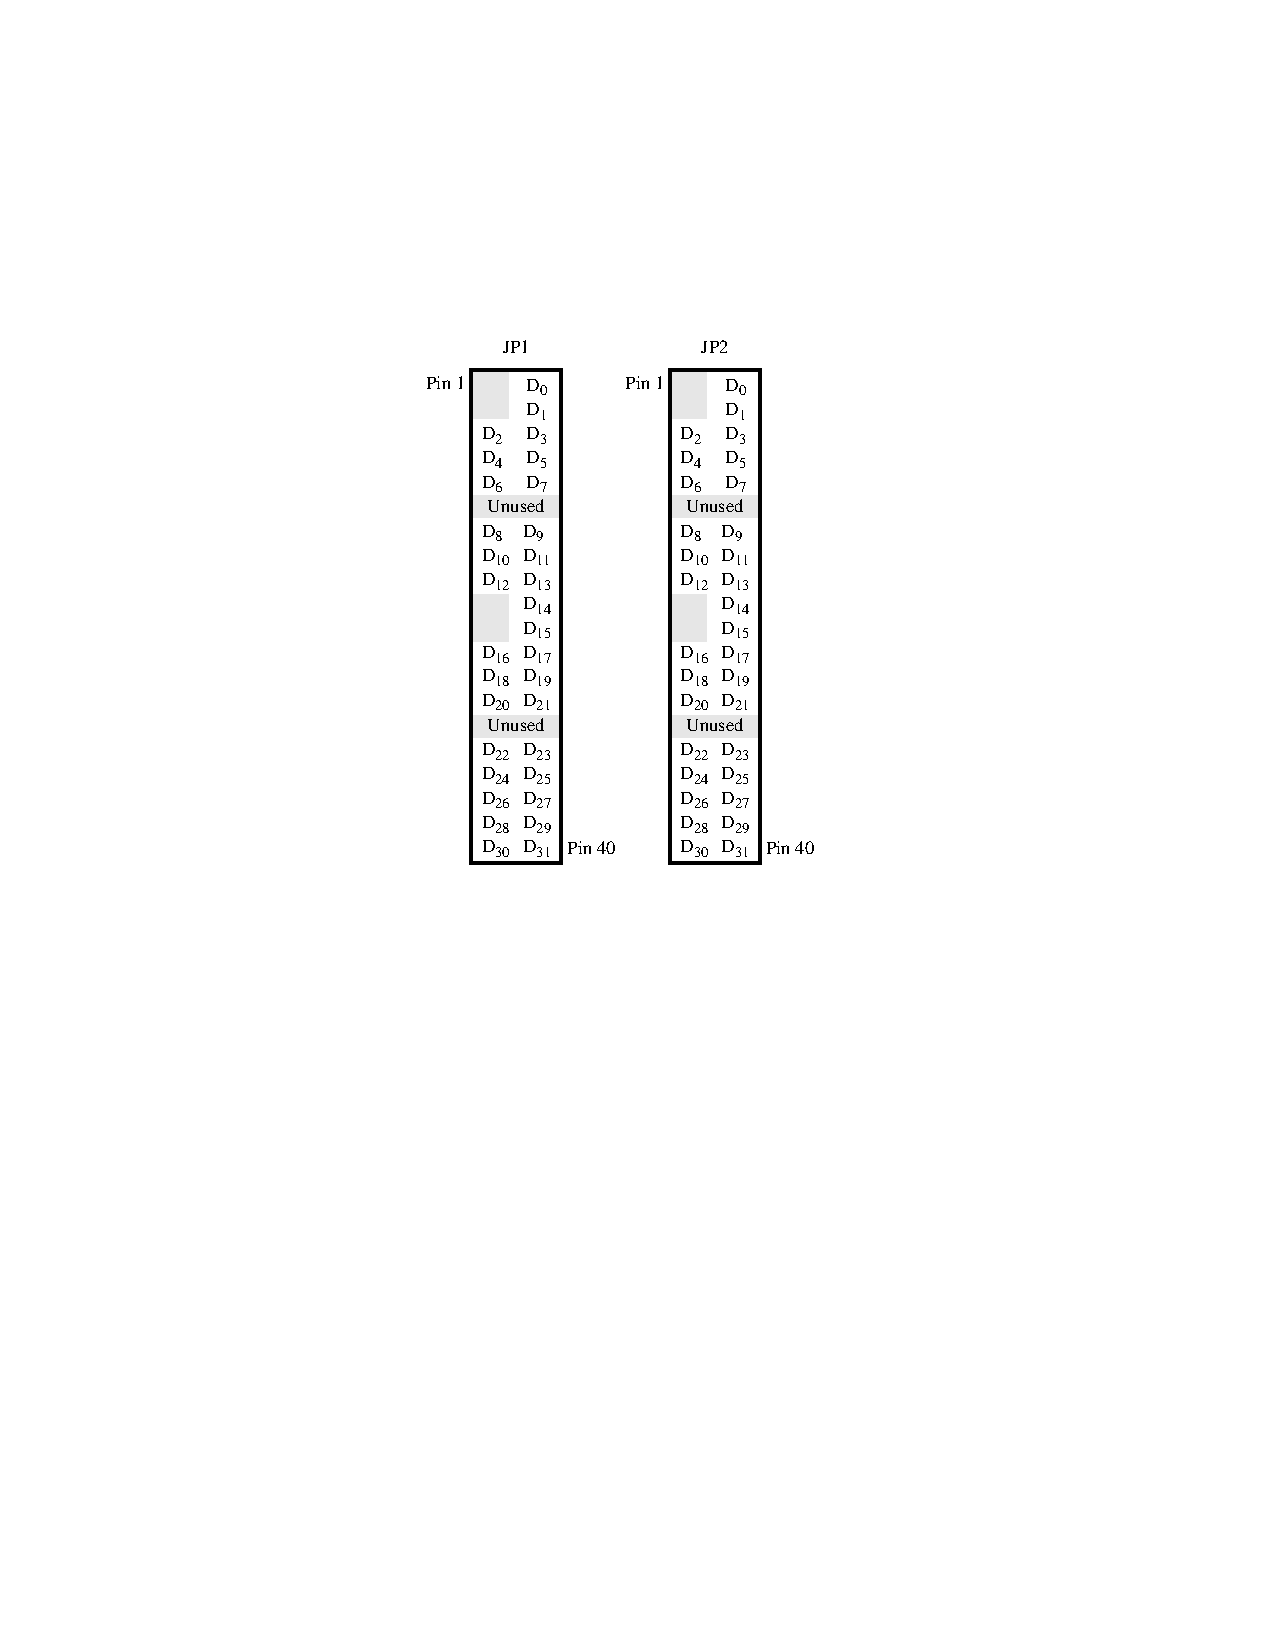
\includegraphics[trim={0 0 0 0.5cm},clip]{../../../common/figs/FPGA_PP_Expansion_Port.pdf}
   \end{center}
	\caption{Assignment of parallel port bits to pins on {\it \expansionPortA} and {\it \expansionPortB}.}
	\label{fig:expansion_port}
\end{figure}

